% Part 1: Determining RecB binding time
\section*{Results}

\subsection*{RecB forms long-lived spots when recruited to cipro\-floxacin DSBs}

\begin{figure*}[htbp]
    \centering
    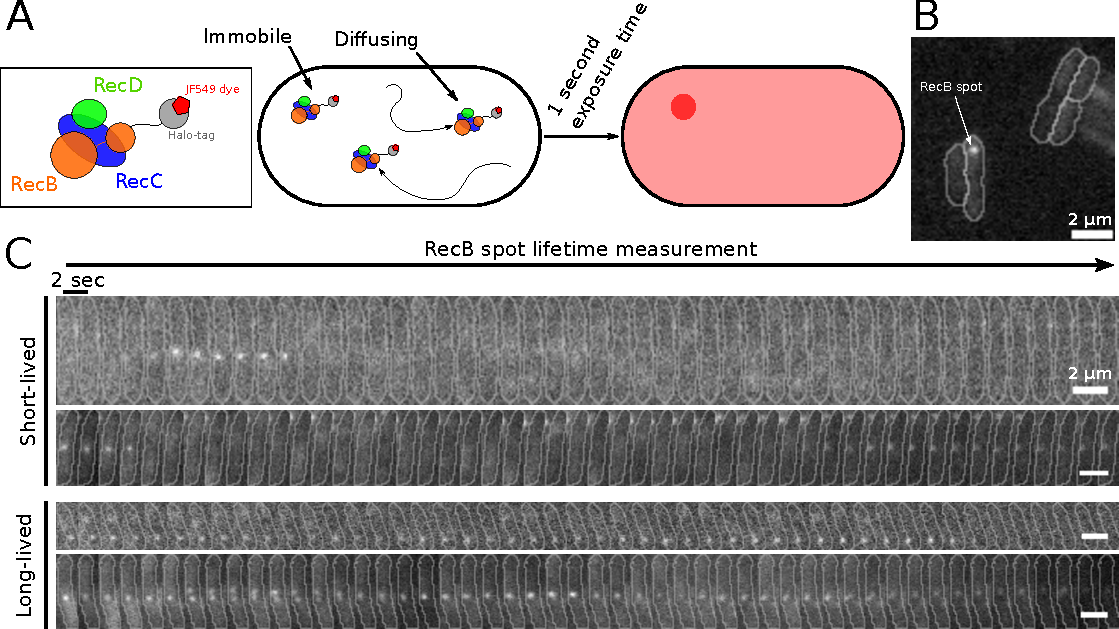
\includegraphics[width=.8\textwidth]{Figures/Fig1_Exp_principle.pdf}
    \caption{Measuring the binding time of RecB on DNA. \textbf{(A)} Scheme of our experimental protocol. The RecB subunit of the RecBCD complex is fused to a Halo-tag, bound by the JF549 fluorescent dye\cite{Lepore2019a, Lepore2023}. A long exposure time (1 sec) makes diffusing molecules appear as diffuse signal in the cell, while DNA-bound molecules are visible as bright, diffraction-limited spots. \textbf{(B)} Example image of a RecB spot (white arrow). \textbf{(C)} Example kymographs of RecB throughout an acquisition, showing short- and long-lived fluorescent spots. A short timelapse (100 sec) is acquired at a different position every 2 min for 75 min.}
    \label{Fig:lifetimes}
\end{figure*}

To quantify RecB binding time to DNA in live \textit{E. coli}, we used a Halo-tag fusion to the RecB subunit, conjugated to the JF549 fluorescent dye (Figure \ref{Fig:lifetimes}A). The fusion was previously used and characterised, ensuring specific one-to-one labelling of RecB molecules without adverse effects on the DNA repair process\cite{Lepore2019a,Lepore2023}. Due to the large size and topological constraints of the bacterial chromosome, DNA-bound RecB diffuses very slowly\cite{Lepore2023}. We therefore applied the previously developed technique of localisation enhancement\cite{Yu2006, Elf2007}: since RecB is present at low copy numbers in \textit{E. coli} ($\sim$5 molecules per cell on average\cite{Lepore2019a}), imaging live cells with a long exposure time (1 second) made fast-diffusing RecB molecules appear as weak homogeneous signal in the cell, while immobile or slow-diffusing RecB molecules formed intense diffraction-limited spots (referred to throughout this article as RecB spots, Figures \ref{Fig:lifetimes}A and \ref{Fig:lifetimes}B). The complete absence of similar spots in cells expressing the free Halo-tag from a plasmid confirmed that these spots were specific to RecB (Supp. Figure \ref{SIFig:freehalo_image}). However, the exact nature of these spots needed to be confirmed. Although DNA-bound molecules are expected to diffuse very slowly, the RecBCD-Halo complex diffuses in the crowded and constrained environment of the cytoplasm, and might undergo transient interactions with DNA\cite{Lepore2023}. These factors could lead to RecB spots forming independently of DNA binding. To gain more insight into the nature of RecB spots, we increased the number of induced DSBs by adding ciprofloxacin to agar pads before imaging, and probed the dynamics of the spots by recording 100-second timelapse videos with 2 sec interval between frames on different positions in the sample, for a total time of 60 min following exposure to ciprofloxacin (Figure \ref{Fig:lifetimes}C). The 1 second exposure time was optimal to detect RecB spots with good signal-to-noise, while limiting dye photobleaching and keeping a sufficient time resolution to determine spot lifetimes. Visual inspection of the timelapse data showed that RecB spot lifetime was hetereogenous, with a majority of spots being visible only for a few frames, and a small number persisting for longer times. These longer-lived spots became more frequent as the ciprofloxacin concentration was increased.

% RecB spot lifetime
Using the timelapse data, we built histograms of RecB spot lifetimes at the different ciprofloxacin concentrations (Figure \ref{Fig:lifetimes}D). In the absence of ciprofloxacin, a large majority of spots lasted less than 10 seconds. Under increasing ciprofloxacin concentrations, the distribution showed a clear shift towards longer-lived spots, with the histogram at 20 and 30 ng/ml ciprofloxacin displaying a clear "tail" of long-lived events ($>$ 10 sec). Fitting these histograms with a mono-exponential decay model ($y = a.e^{-k.t}$) did not match the experimental data accurately (Supp. Figure \ref{SIFig:monoexp_fits}). In particular, it did not account for the distribution tail of longer-lived spots that formed at high ciprofloxacin concentrations. Fitting with a bi-exponential decay model ($y = a_1.e^{-k_1.t} + a_2.e^{-k_2.t}$) accounted better for the longer-lived RecB spots (Figure \ref{Fig:lifetimes}D). The bi-exponential fit outlined two populations of spots with different lifetimes: a short-lived one, with average lifetimes ranging from 1.4 to 1.7 sec, and a longer-lived one, with average lifetimes ranging from 10 to 14 sec (Table \ref{tab:fit_results}). Even though the short-lived spots always represented a majority of events (over 90\% of the spots), the proportion of long-lived spots tended to increase under higher ciprofloxacin exposure (from 1.4\% $\pm$ 0.3 under 3 ng/ml ciprofloxacin to 5.5\% $\pm$ 1.4 under 30 ng/ml ciprofloxacin).

\begin{figure*}[htbp]
    \centering
    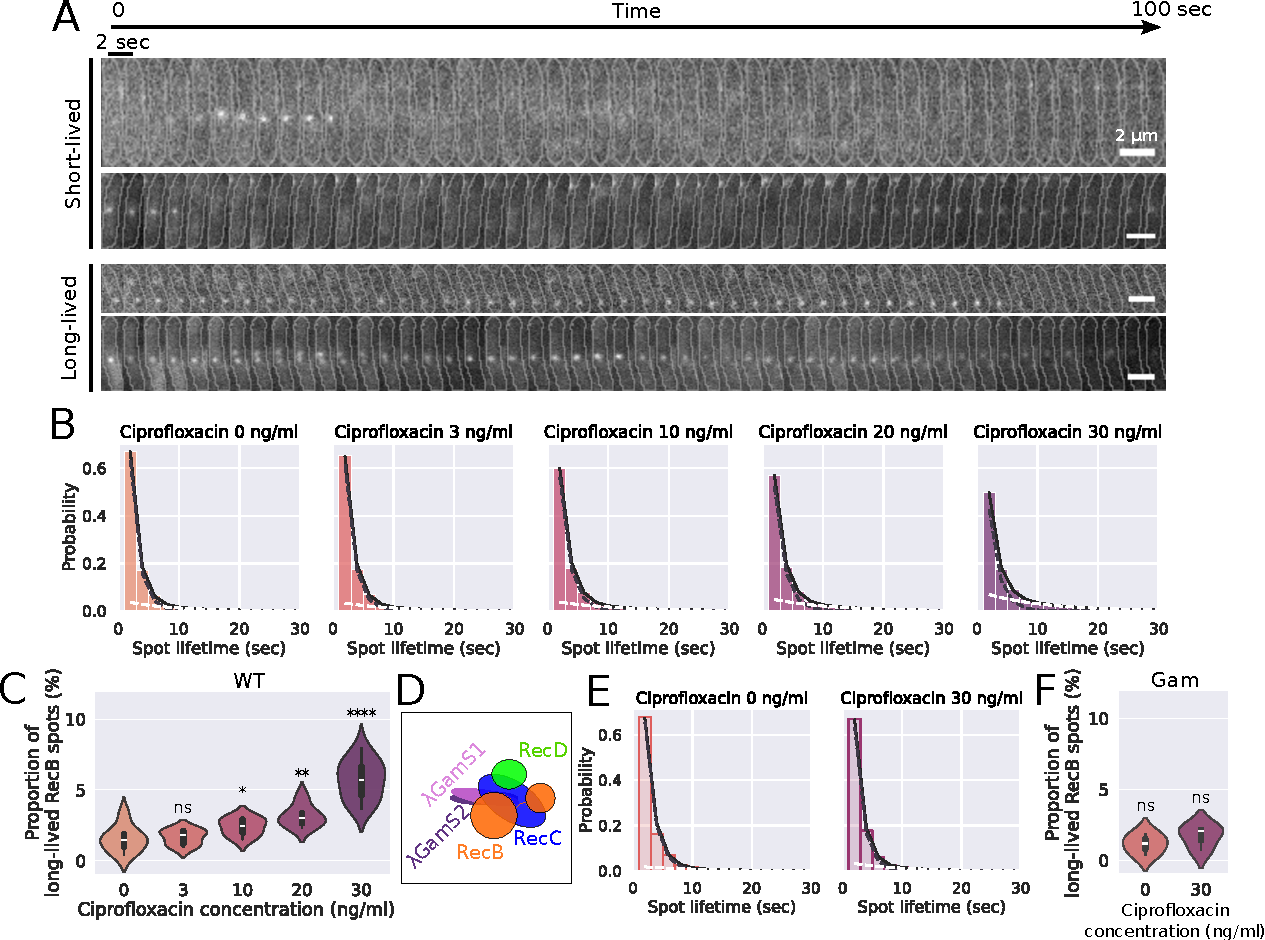
\includegraphics[width=.8\textwidth]{Figures/Fig2_RecB_lifetime.pdf}
    \caption{RecB lifetime on DNA under ciprofloxacin exposure. \textbf{(A)} RecB spot lifetime histograms at 0, 3, 10, 20 and 30 ng/ml ciprofloxacin (bars), fitted with a bi-exponential decay model (black line, fit components showed as dashed lines). \ncells{66,764}. \nspots{170,138}. \textbf{(B)} RecB spot lifetime histograms (bars) for cells over-expressing the Gam protein, fitted with a bi-exponential decay model (black line, fit components showed as dashed lines). \ncells{8,812}. \nspots{18,698}. \textbf{(C)} Probability of a spot corresponding to a DNA-bound RecB molecule, for cells over-expressing the Gam protein. Black dots show individual datasets, the black line is the average between them, and the red dashed line shows the smallest lifetime at which RecB spots have 95\% probability to be DNA-bound. \ncells{8,812}. \nspots{18,698}. \textbf{(D)} Representative defocussed brightfield images of wild-type (WT), \dreca\ and \geneteneighty\ mutants cells, in the absence and presence of ciprofloxacin (30 ng/ml).}
    \label{Fig:recruitment}
\end{figure*}

\begin{table}[htbp]
    \centering
    \caption{Parameters derived from the spot lifetime histogram fits (Figures \ref{Fig:lifetimes}D and \ref{Fig:recruitment}B). The lifetime was calculated as the inverse of the fitted dissociation rate. Values are given as the median $\pm$ standard deviation over at least 3 independent datasets. \ncells{66,764}. \nspots{170,138}}
    \begin{tabular}{llll}
        \toprule
         &  & Lifetime (sec) & Population (\%) \\
        Ciprofloxacin & Type &  &  \\
        \midrule
        \multirow[t]{2}{*}{0 ng/ml} & Short & 1.4 $\pm$ 0.2 & 98.2 $\pm$ 1.0 \\
         & Long & 9.5 $\pm$ 9.7 & 1.8 $\pm$ 1.0 \\
        \cline{1-4}
        \multirow[t]{2}{*}{3 ng/ml} & Short & 1.5 $\pm$ 0.1 & 98.6 $\pm$ 0.3 \\
         & Long & 10.5 $\pm$ 1.3 & 1.4 $\pm$ 0.3 \\
        \cline{1-4}
        \multirow[t]{2}{*}{10 ng/ml} & Short & 1.7 $\pm$ 0.2 & 97.6 $\pm$ 0.6 \\
         & Long & 13.7 $\pm$ 2.3 & 2.4 $\pm$ 0.6 \\
        \cline{1-4}
        \multirow[t]{2}{*}{20 ng/ml} & Short & 1.6 $\pm$ 0.2 & 96.6 $\pm$ 0.8 \\
         & Long & 11.8 $\pm$ 2.1 & 3.4 $\pm$ 0.8 \\
        \cline{1-4}
        \multirow[t]{2}{*}{30 ng/ml} & Short & 1.7 $\pm$ 0.2 & 94.5 $\pm$ 1.4 \\
         & Long & 13.3 $\pm$ 2.2 & 5.5 $\pm$ 1.4 \\
        \cline{1-4}
        \midrule
        \multirow[t]{2}{*}{0 ng/ml, Gam} & Short & 1.7 $\pm$ 0.2 & 99.2 $\pm$ 0.4 \\
         & Long & 15.5 $\pm$ 9.1 & 0.8 $\pm$ 0.4 \\
        \cline{1-4}
        \multirow[t]{2}{*}{30 ng/ml, Gam} & Short & 1.5 $\pm$ 0.1 & 98.2 $\pm$ 0.9 \\
        & Long & 8.2 $\pm$ 1.8 & 1.8 $\pm$ 0.9 \\
        \bottomrule
        \end{tabular}
    \label{tab:fit_results}
\end{table}

% Gam
To determine whether short- or long-lived spots resulted from RecB binding to DNA leading to SOS induction, we measured RecB spot lifetime in the presence and absence of ciprofloxacin while over-expressing the Gam protein of phage $\lambda$ from a plasmid. The Gam protein was previously shown to bind in place of DNA on the RecBCD complex\cite{Wilkinson2016}, and its overexpression is expected to abolish RecBCD binding to DSBs. Accordingly, cells that over-expressed Gam and were exposed to high ciprofloxacin (30 ng/ml) showed little elongation compared to cells that did not overexpress Gam (Supp. Figure \ref{SIFig:Gam_cell_length}), indicating that most cells did not induce the SOS response, due to the inability of the RecBCD-Gam complex to bind to DSBs and load RecA. The resulting RecB spot lifetimes showed a similar distribution to the one obtained in the absence of ciprofloxacin (Supp. Figure \ref{SIFig:Gam_RecB_lifetimes_fits}). This was confirmed by fitting the histogram with our bi-exponential decay model, which found a proportion of long-lived spots in the presence of 30 ng/ml ciprofloxacin (1.8\% $\pm$ 0.9, Table \ref{tab:fit_results}) equivalent to wild-type cells that were not exposed to ciprofloxacin (1.8\% $\pm$ 1). The residual amount of long-lived RecB spots in the presence of Gam could be due to residual DNA binding despite the presence of Gam. This residual binding could also be the cause for the small increase in cell length observed in Gam-expressing cells under 30 ng/ml ciprofloxacin (Supp. Figure \ref{SIFig:Gam_cell_length}). Since Gam overexpression prevents RecB binding to DNA ends, and specifically caused long-lived spots to disappear, we can conclude that long-lived spots correspond to RecB molecules that have bound to DNA. Given that under Gam overexpression, 95\% of RecB spots were shorter than 10 sec (Figure \ref{Fig:recruitment}A), we considered any spot with a lifetime over 10 sec to be a DNA-bound RecB molecule. The appearance of short-lived spots in the presence of Gam is likely due to a combination of short-lived DNA binding and slow, confined diffusion of the RecBCD-Gam-Halo complex (Supp. Note \ref{note:spurious_spots} and Supp. Figure \ref{SIFig:displacement_simul}). Therefore, spots that are visible for less than 10 seconds cannot be reliably assigned as either DNA-bound or not. However, the largely reduced cell elongation in the presence of Gam (\ref{SIFig:Gam_cell_length}) indicates that short-lived spots do not trigger the SOS response.

Using the Gam protein allowed us to identify DNA-bound RecB molecules as the longer-lived population in our bi-exponential fits of the RecB spot lifetime histograms. We determined that when it processes a DSB, RecB stays bound to DNA for 10 to 15 seconds on average, regardless of the ciprofloxacin concentration. To test whether the duration of ciprofloxacin exposure had an effect on spot lifetimes, we performed separate fits at 15 min intervals (Supp. Figure \ref{SIFig:RecB_lifetimes_timepoints}). The RecB spot lifetimes obtained were consistent with those reported in Table \ref{tab:fit_results}: 10-15 sec for long-lived spots, and 1.5-2 sec for short-lived spots.

% Effect of ciprofloxacin exposure on the different mutants
Imaging RecB binding to DSBs in the presence of different concentrations of ciprofloxacin allowed us to determine that the amount of DNA damage experienced by the cells did not influence the time spent by RecB on DNA (Table \ref{tab:fit_results}). This is consistent with processing of DSBs by RecBCD taking place independently of the presence of other DSBs in the cell. Next, we wanted to test whether RecB dissociation from DNA was influenced by the following step in the repair process, the loading of RecA on DNA. Therefore, we imaged the \dreca\ and \geneteneighty\ mutants in the presence and absence of 30 ng/ml ciprofloxacin. Figure \ref{Fig:mutants}A shows defocussed brightfield images of cells that were not exposed to ciprofloxacin, and cells that were exposed to 30 ng/ml ciprofloxacin for 60 min. Supp. Figure \ref{SIFig:mutants_cell_lengths} shows the average cell lengths in the different conditions and ciprofloxacin exposure durations. As previously observed, wild-type cells show a clear response to exposure to 30 ng/ml ciprofloxacin, where the cell length increases significantly due to induction of the SOS response. In contrast to this, since the \dreca\ mutant is unable to form a RecA filament, it is also unable to induce the SOS response. Cell length therefore remains unchanged, even upon prolonged exposure to 30 ng/ml ciprofloxacin. In the absence of ciprofloxacin, the \geneteneighty\ mutant cells were slightly more elongated than wild-type cells. This matches previous indications that this mutant has a higher baseline of SOS induction than wild-type cells in the absence of exogenous DNA damage\cite{Lepore2023}. Upon exposure to ciprofloxacin, the cell length of the \geneteneighty\ mutant increased, albeit slightly less on average than the wild-type's (Supp. Figure \ref{SIFig:mutants_cell_lengths}). This might be a reflection of \teneighty's inability to directly load RecA on the DNA, and the use of the alternative RecFOR pathway leading to different time dynamics of the SOS response\cite{Ivancic-Bace_2003,Lepore2023}.

% RecB binding time in the mutants
As for the wild-type strain, we imaged RecB, computed histograms of RecB spot lifetimes and fitted them with a bi-exponential decay model (Supp. Figure \ref{SIFig:mutants_biexp_fits}), from which we extracted the binding times of RecB on DNA (Figure \ref{Fig:mutants}B). In the \dreca\ mutant, the DNA-binding lifetime of RecB was similar to the wild-type ($\sim$10 sec), both in the presence and absence of ciprofloxacin. This suggests that RecA loading by RecBCD does not play a role in triggering the dissociation of wild-type RecBCD from DNA. In contrast, \teneighty\ stayed bound to DNA for longer on average than wild-type RecB ($\sim$16 sec). This could be due to the inability of \teneighty\ to digest the DNA it unwinds, making dissociation more challenging due to the DNA strands threading through the RecBCD complex.

% Table 2: RecB spot lifetime in the mutants
\begin{table*}[htbp]
    \centering
    \caption{Parameters derived from the spot lifetime histogram fits for the \dreca\ and \geneteneighty\ strains (Supp. Figure \ref{SIFig:mutants_biexp_fits}). The lifetime was calculated as the inverse of the fitted dissociation rate. Values are given as the median $\pm$ standard deviation over at least 3 independent datasets. \ncells{56,131}. \nspots{177,646}.}
    \begin{tabular}{lllll}
        \toprule
        &  &  & Lifetime (sec) & Population (\%) \\
        Strain & Ciprofloxacin & Type &  &  \\
        \midrule
        \multirow[t]{4}{*}{\dreca} & \multirow[t]{2}{*}{0 ng/ml} & Short & 1.76 $\pm$ 0.16 & 96.55 $\pm$ 1.01 \\
        &  & Long & 12.96 $\pm$ 1.78 & 3.45 $\pm$ 1.01 \\
        \cline{2-5}
        & \multirow[t]{2}{*}{30 ng/ml} & Short & 2.11 $\pm$ 0.22 & 90.47 $\pm$ 3.37 \\
        &  & Long & 12.38 $\pm$ 3.48 & 9.53 $\pm$ 3.37 \\
        \cline{1-5} \cline{2-5}
        \multirow[t]{4}{*}{$recB_{1080}$} & \multirow[t]{2}{*}{0 ng/ml} & Short & 1.75 $\pm$ 0.16 & 97.37 $\pm$ 0.85 \\
        &  & Long & 16.65 $\pm$ 5.52 & 2.63 $\pm$ 0.85 \\
        \cline{2-5}
        & \multirow[t]{2}{*}{30 ng/ml} & Short & 2.12 $\pm$ 0.06 & 96.49 $\pm$ 0.69 \\
        &  & Long & 19.4 $\pm$ 7.06 & 3.51 $\pm$ 0.69 \\
        \bottomrule
    \end{tabular}
    \label{tab:fit_mutants}
\end{table*}

% Part 2: Rate of recruitment of RecB on the DNA
\begin{figure}[htbp]
    \centering
    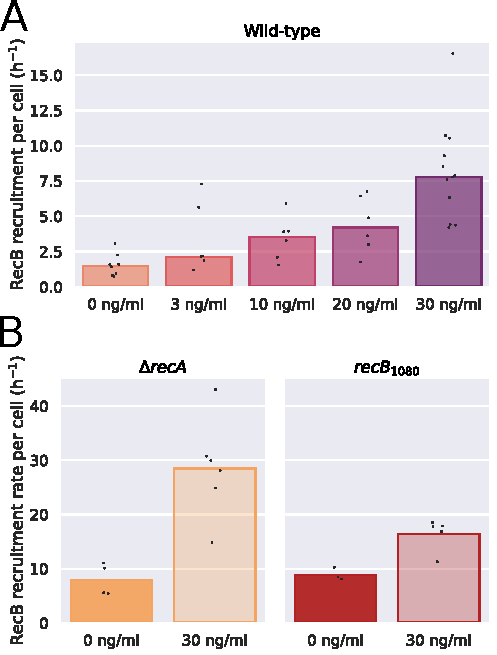
\includegraphics[width=.4\textwidth]{Figures/Fig3_RecB_recruitment.pdf}
    \caption{\textbf{(A)} Recruitment rate per cell of RecB on DNA at different ciprofloxacin concentrations. Black points show individual datasets, and bars the median value. \ncells{66,764}. \nspots{170,138}. \textbf{(B)} Recruitment rate per cell of RecB on DNA for the \dreca\ and \geneteneighty\ mutants. Black points show individual datasets, and bars the median value. \ncells{23,540}. \nspots{99,891}.}
    \label{Fig:recb_recruitment}
\end{figure}

% RecB recruitment in WT
Whereas the lifetime of the fluorescent spots informs us on how long RecB stays bound to DNA, the rate of appearance of spots helps us estimate the rate of recruitment of RecB to DSBs under each DNA damage condition (Figure \ref{Fig:recruitment}B). To do so, we used the RecB spot lifetime histogram fits to estimate the total number of slow-dissociating spots per timelapse. Since we determined that the appearance of a slow-dissociating spot corresponds to the binding of RecB to a DSB, this allowed us to calculate the number of RecB recruitments to DSBs per cell per hour. We estimated that under endogenous damage or low ciprofloxacin concentrations, 1 to 2 RecB molecules are recruited to the DNA per hour on average. This is roughly consistent with the previous estimate of 18\% of cells generating an endogenous DSB per cell cycle\cite{Sinha2018}. At ciprofloxacin concentrations above the MIC (30 ng/ml), the recruitment rate increased to an average of 8 RecB recruited to DNA per hour. Furthermore, we expect that this recruitment rate gives a close estimate of the rate of formation of DSBs by ciprofloxacin (see discussion).

% RecB recruitment in mutants
Estimating the recruitment rate of RecB to DNA provided additional insight into the dynamics of DSB processing in the \dreca\ and \geneteneighty\ mutants (Figure \ref{Fig:mutants}C). In the \dreca\ mutant, the rate of recruitment of RecB was increased compared to wild-type cells, both in the presence and absence of ciprofloxacin (Figure \ref{Fig:mutants}C). As in both cases the rate of DSB formation is expected to be the same between the wild-type and the \dreca\ mutant, we can hypothesise that this higher rate of RecB recruitment to DNA is due to multiple recruitment events on the same original DSB that cannot be repaired. In the mutant cells, RecBCD processes the DNA, but the generated ssDNA cannot be coated with the RecA protein, and is therefore likely to be degraded by cellular endo- and exonucleases such as SbcCD and ExoI\cite{Zahradka2009}. Degradation of the ssDNA would lead to a blunting of the DNA end, hence creating a new substrate for RecBCD binding. This deleterious cycle was previously reported to occur in cells lacking the RecA protein, eventually leading to full chromosome degradation\cite{Capaldo1975,Skarstad1993}. In our experiment, it results in multiple recruitments of RecB to DNA for each DSB.

% Recruitment in RecB1080
In the \geneteneighty\ mutant, RecB recruitment is higher than in WT cells, but equivalent (in the absence of ciprofloxacin) or lower (in the presence of 30 ng/ml ciprofloxacin) to the level of RecB recruitment in the \dreca\ mutant (Figure \ref{Fig:mutants}C). Upon DSB recognition, \teneighty\ unwinds DNA without digesting it, and dissociates $\sim$1.5 times slower than wild-type RecB (Figure \ref{Fig:mutants}B). After RecBCD dissociation, we expect two competing pathways to take place. Either (i) the unwound ssDNA is digested by cellular endo- and exonucleases, creating a new RecBCD substrate; or (ii) RecFOR displaces the SSB (Single-Strand DNA-Binding) protein and promotes RecA loading, allowing DNA repair by homologous recombination to proceed\cite{Ivancic-Bace_2003}. As a result, \teneighty can be recruited on DNA several times for each DSB (similarly to the \dreca\ mutant), but the cycle of re-recruitment can be broken by the action of RecFOR.


% Part 3: Colocalisation of RecB with the nucleoid (to be reviewed/adjusted)
\begin{figure*}[htbp]
    \centering
    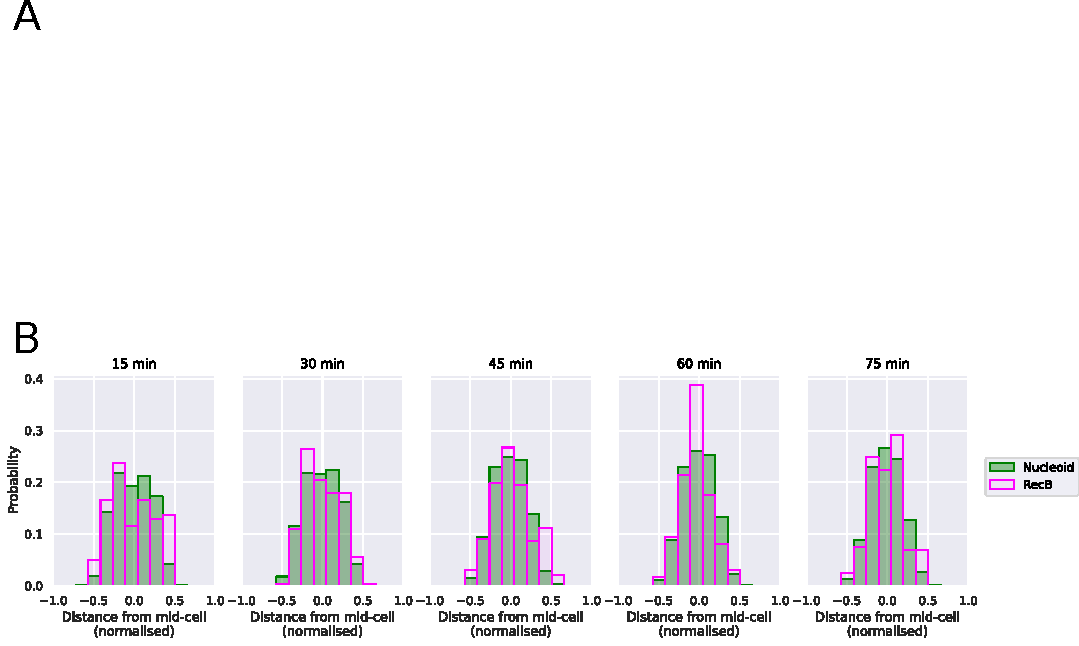
\includegraphics[width=.8\textwidth]{Figures/Fig4_nucleoid.pdf}
    \caption{Colocalisation of RecB spots with the bacterial nucleoid. \textbf{(A)} Representative images of cells (segmented outline in grey) showing the nucleoid (green) and RecB-associated fluorescence (magenta). RecB spots (indicated by arrows) are located in close proximity to the nucleoid. \textbf{(B)} Overlay of nucleoid density (green area) and position of DNA-bound RecB molecules (magenta bars) along the cell's long axis, for different ciprofloxacin concentrations (0 to 30 ng/ml). \ncells{24,014}. \nspots{79,969}. \nnucl{31,441}. \textbf{(C)} Representative overlay images of RecB-associated fluorescence (magenta) and the bacterial nucleoid (green) in the \dreca\ and \geneteneighty\ mutants. Segmented cell outline shown in grey. \textbf{(D)} Overlay of nucleoid density (green area) and position of DNA-bound RecB molecules (magenta bars) along the cell's long axis for the \dreca\ and \geneteneighty\ mutants. \ncells{7,804}. \nspots{36,595}. \nnucl{11,215}.}
    \label{Fig:nucleoid}
\end{figure*}

% Nucleoid imaging
In \emph{E. coli}, the loading of RecA on DNA triggers the SOS response, which inhibits cell division, leading to cell filamentation. Previous studies have reported that the SOS response also triggers compaction of the bacterial nucleoid\cite{Odsbu2014}. To see if this was the case for breaks induced by ciprofloxacin in our experimental conditions, we stained DNA using the Sytox Green dye. The use of a green dye allowed us to concomitantly image RecB, and to correlate the position of DNA-bound RecB molecules with that of the nucleoid. Figure \ref{Fig:reca_nucleoid}C shows representative images of the nucleoid and DNA-bound RecB after 60 minutes of exposure to different concentrations of ciprofloxacin. In untreated cells, the nucleoid was often observed to be bi-lobed, consistently with previous observations\cite{Lepore2023}. After exposure to ciprofloxacin, the cells appeared elongated, and the nucleoid was often compacted in the centre of the cell. Due to nucleoid compaction, the total fraction of the cell occupied by the nucleoid decreased, from 40\% on average in untreated cells to 31\% in cells exposed to 30 ng/ml of ciprofloxacin for an hour (Supp. Figure \ref{SIFig:nucleoid_compaction}). This compaction was accompanied by a centring of the nucleoid along the cell's long axis. Supp. Figure \ref{SIFig:nucleoid_position} shows that upon increasing exposure to ciprofloxacin (in time and concentration), the cells elongate, and nucleoids were increasingly centred.

% Correlation of nucleoid and RecB spots
As expected, DNA-bound RecB were found in close proximity to the nucleoid (Figure \ref{Fig:reca_nucleoid}C). Figure \ref{Fig:reca_nucleoid}D shows the strong overlap between the spatial distribution of DNA-bound RecB spots and the nucleoid density in the cell (Supp. Figure \ref{SIFig:recb_nucleoid_timepoints} shows the same data after different durations of ciprofloxacin exposure). Due to nucleoid compaction and centring, both the nucleoid density and the position of DNA-bound RecB remained within $\sim$2 µm either side of the cell centre, despite the cells having elongated significantly.

% Compaction of the nucleoid in mutants
The differences in induction of the SOS response between the wild-type cells and the mutants resulted in different states of compaction for the bacterial nucleoid (Figure \ref{Fig:mutants}D, Supp. Figure \ref{SIFig:mutants_nucleoid_compaction}). Whereas in the wild-type, exposure to ciprofloxacin triggered compaction and centring of the nucleoid, the inability of the \dreca\ mutant to induce the SOS response resulted in two separate nucleoid regions at the cell poles. Despite the absence of SOS induction, the nucleoid occupied a smaller fraction of the cell in the \dreca\ mutant after exposure to ciprofloxacin (Supp. Figure \ref{SIFig:mutants_nucleoid_compaction}). This can be attributed to the progressive degradation of the bacterial chromosome by the repeated cycles of RecBCD binding\cite{Capaldo1975,Skarstad1993}. In the RecB1080 mutant, the nucleoid appeared more disorganised than in wild-type cells (Figure \ref{Fig:mutants}D), but still underwent compaction at the centre of the cell upon exposure to ciprofloxacin (Supp. Figure \ref{SIFig:mutants_nucleoid_compaction}). Notably, the level of compaction of the nucleoid was slightly less important than in wild-type cells (38\% $\pm$ 9 of the cell occupied by the nucleoid after 75 min of exposure to ciprofloxacin, against 32\% $\pm$ 11 in the wild-type). This might again be a reflection of the less efficient RecA loading in this mutant, leading to different time dynamics of the SOS induction.

% Colocalisation of RecB with the nucleoid in mutants
In all three strains, the localisation of DNA-bound RecB overlapped with the bacterial nucleoid, consistent with RecB being recruited to DSBs (Figures \ref{Fig:mutants}D and \ref{Fig:mutants}E). In the \dreca\ mutant, addition of 30 ng/ml ciprofloxacin did not change the spatial distribution of nucleoid density or DNA-bound RecB. This is consistent with \dreca\ cells being unable to induce the SOS response, and therefore not undergoing nucleoid compaction. In the \geneteneighty\ mutant, both nucleoid density and DNA-bound RecB distributions form a single peak at the cell centre, in the presence and absence of ciprofloxacin. This is consistent with the \geneteneighty\ mutant having a higher baseline of SOS induction than wild-type cells, as previously reported\cite{Lepore2023}. The slightly broader distribution of nucleoid density and DNA-bound RecB position in the \geneteneighty\ mutant exposed to ciprofloxacin compared to the wild-type is consistent with the lesser nucleoid compaction observed in this mutant (Supp. Figure \ref{SIFig:mutants_nucleoid_compaction}).

% Part 4: Imaging RecA foci and filaments (to be moved to the end)
\subsection*{Ciprofloxacin exposure induces formation of RecA filaments and nucleoid compaction}

%% RecA imaging
During processing of DSBs, RecBCD facilitates the loading of the RecA protein on single-stranded DNA. To broaden our view of the repair process downstream of RecBCD, we imaged a tandem fusion of RecA with the fluorescent protein SYFP2\cite{Wiktor2021}. Based on the fluorescence distribution in the cells (Figure \ref{Fig:reca_nucleoid}A), we identified three states of RecA: diffuse, forming a bright focus, or forming an elongated filament, which matches previous \emph{in-vivo} observations of RecA\cite{Wiktor2021}. Because of the large diversity of shapes observed, especially for RecA filaments, the detection of RecA structures by rule-based algorithms was challenging. Therefore, we designed and trained a deep-learning algorithm capable of classifying individual cells based on the three types of spatial distributions cited above (Figure \ref{Fig:reca_nucleoid}B, Supp. Figure \ref{SIFig:object_class}). In cells that were not exposed to ciprofloxacin, the RecA-associated fluorescence was mostly diffuse, and occasionally formed a bright focus. This is consistent with cells undergoing occasional endogenous DNA damage. The proportion of cells that contained RecA filaments was low in the absence of ciprofloxacin ($\sim$10\%). After one hour of exposure, the proportion of cells that contained a RecA filament had increased to $\sim$40\% at 20 ng/ml ciprofloxacin, and $\sim$60\% at 30 ng/ml. RecA foci on the other hand formed quickly following ciprofloxacin exposure (present in $\sim$40\% of the cells after 15 min of exposure to 30 ng/ml ciprofloxacin) and came back to endogenous damage level after $\sim$1 hour. Taken together, these results show that RecA foci are transient structures in the repair process that do not accumulate under high DNA damage, whereas RecA filaments accumulate under constant exposure to ciprofloxacin.



% \begin{figure*}[htbp]
%     \centering
%     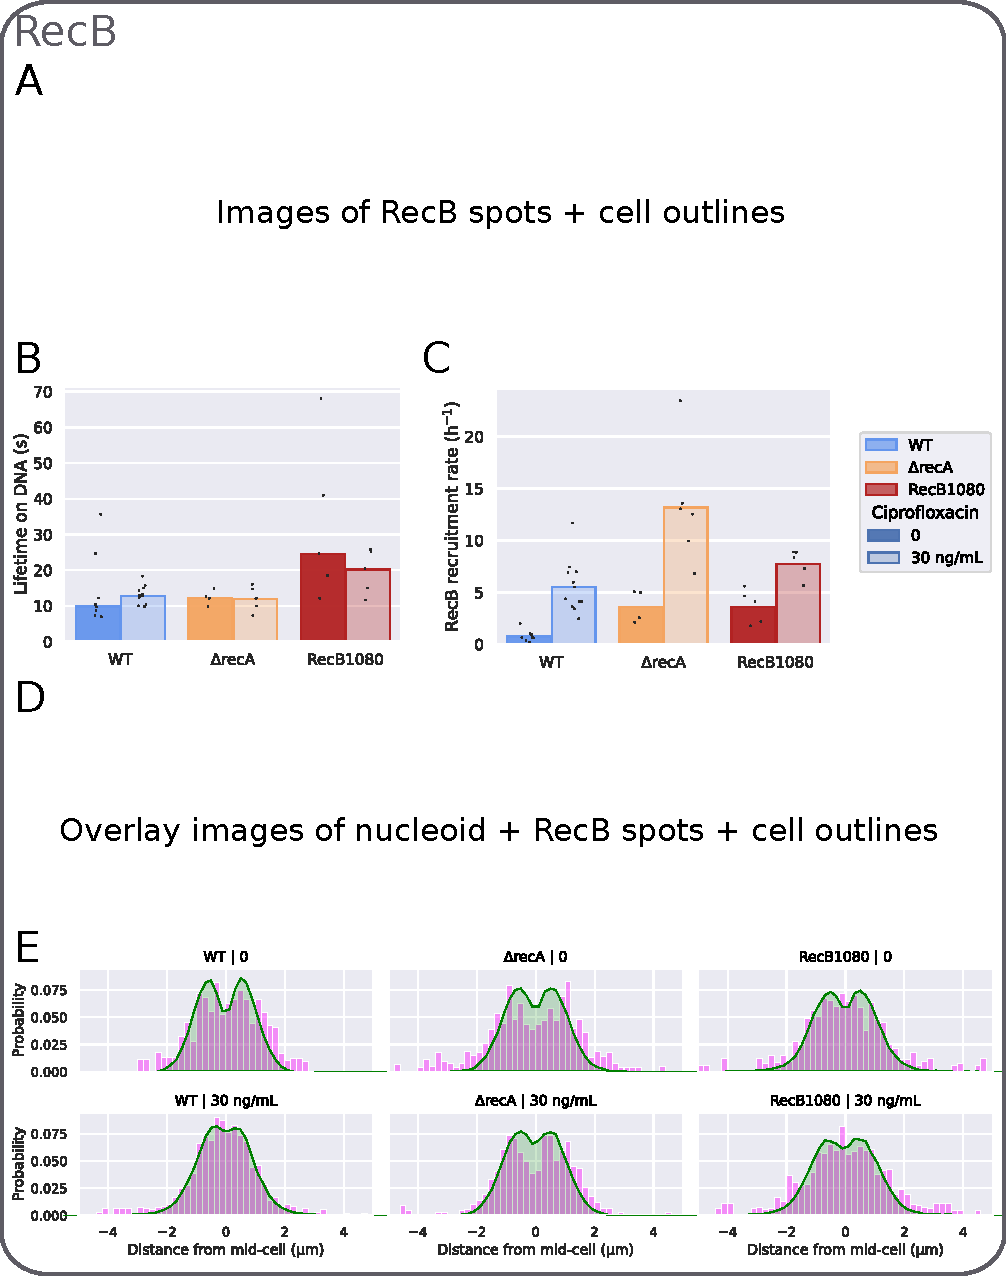
\includegraphics[width=.75\textwidth]{Figures/Fig4_mutants.pdf}
%     \caption{RecB binding to DNA in the \dreca\ and \geneteneighty\ mutant strains in the absence and presence of ciprofloxacin (30 ng/ml). \textbf{(A)} Representative brightfield images of wild-type (WT), \dreca\ and \geneteneighty\ mutants cells, in the presence and absence of ciprofloxacin (30 ng/ml). \textbf{(B)} Fitted lifetimes of RecB molecules on DNA. Black dots show individual datasets, and bars the median values. \ncells{56,131}. \nspots{177,646}. \textbf{(C)} Rate of recruitment of RecB to the DNA. Black dots show individual datasets, and bars the median values. \ncells{56,131}. \nspots{177,646}. \textbf{(D)} Representative overlay images of RecB-associated fluorescence (magenta) and the bacterial nucleoid (green). Segmented cell outline shown in grey. \textbf{(E)} Overlay of nucleoid density (green area) and position of DNA-bound RecB molecules (magenta bars) along the cell's long axis. \ncells{15,029}. \nspots{58,331}. \nnucl{20,831}.}
%     \label{Fig:mutants}
% \end{figure*}


% \begin{figure*}[htbp]
%     \centering
%     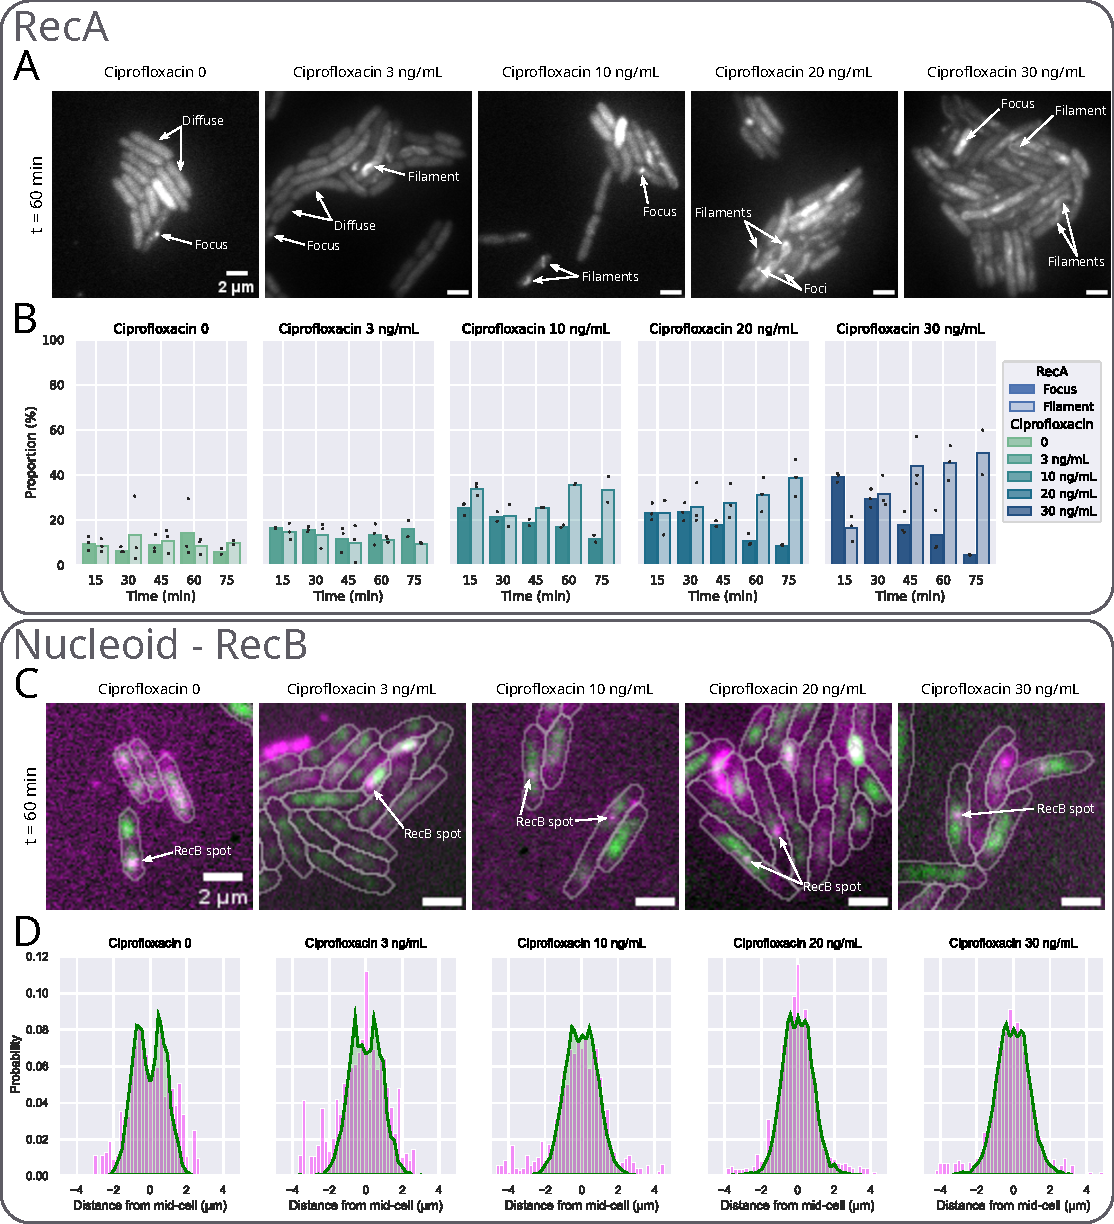
\includegraphics[width=.8\textwidth]{Figures/Fig3_cell_response.pdf}
%     \caption{Bacterial cell response to the induction of DSBs by ciprofloxacin. \textbf{(A)} Representative images of cells containing different RecA structures (diffuse fluorescence, foci or filaments) after 60 minutes of exposure to ciprofloxacin. Arrows point to representative examples of each of these structures. \textbf{(B)} Proportion of cells containing RecA foci or filaments. Black dots represent individual datasets, and bars the average between them. \ncells{32,031}. \textbf{(C)} Representative images of cells (segmented outline in grey) showing the nucleoid (green) and RecB-associated fluorescence (magenta). RecB spots (indicated by arrows) are located in close proximity to the nucleoid. \textbf{(D)} Overlay of nucleoid density (green area) and position of DNA-bound RecB molecules (magenta bars) along the cell's long axis, for different ciprofloxacin concentrations (0 to 30 ng/ml). \ncells{24,014}. \nspots{79,969}. \nnucl{31,441}.}
%     \label{Fig:reca_nucleoid}
% \end{figure*}